\documentclass{article}

%% Language and font encodings
\usepackage[T1]{fontenc}
\usepackage[utf8x]{inputenc}
\usepackage[english]{babel}

\usepackage[colorlinks=true, allcolors=blue]{hyperref}

\urlstyle{tt}
\newcommand{\email}[1]{\href{mailto:#1}{\tt{\nolinkurl{#1}}}}
\newcommand{\orcid}[1]{ORCID: \href{https://orcid.org/#1}{\tt{\nolinkurl{#1}}}}

\usepackage[sfdefault,lf]{carlito}
%% The 'lf' option for lining figures
%% The 'sfdefault' option to make the base font sans serif
\usepackage[parfill]{parskip}
\renewcommand*\oldstylenums[1]{\carlitoOsF #1}
\usepackage{fancyhdr}
\usepackage{natbib}
\usepackage{authblk}
\setlength{\headheight}{41pt}

%% Sets page size and margins
\usepackage[letterpaper,top=3cm,bottom=2cm,left=3cm,right=3cm,marginparwidth=1.75cm]{geometry}

%% Useful packages
\usepackage{amsmath}
\usepackage{graphicx}
\usepackage{booktabs}

\usepackage[colorinlistoftodos]{todonotes}

\usepackage[nolist,nohyperlinks]{acronym}
\usepackage{subcaption}


%\renewcommand{\headrulewidth}{0pt}
\fancyhead[L]{Posted: \today}
\fancyhead[R]{
}
\pagestyle{plain}
\title{A Tool for Automatic Anatomical \& Functional Labeling of Brain Activity Maps}
\author[1,2,*]{Mustafa S. Salman}
\author[3]{Tor D. Wager}
\author[1]{Eswar Damaraju}
\author[1]{Vince D. Calhoun}
\affil[1]{Tri-Institutional Center for Translational Research in Neuroimaging and Data Science (TReNDS), Georgia State University, Georgia Institute of Technology, and Emory University, Atlanta, GA}
\affil[2]{School of Electrical \& Computer Engineering, Georgia Institute of Technology, Atlanta, GA}
\affil[3]{Department of Psychology \& Neuroscience, University of Colorado Boulder, Boulder, CO}
\affil[*]{Corresponding author: \email{esalman@gatech.edu}}
\date{}

\begin{document}
\maketitle
\thispagestyle{fancy}

\begin{abstract}

\end{abstract}

\section{Introduction}

[group ICA]

[FNC]

[artifact detection]

[falff and dyn range]

[REST toolbox masks]

[anatomical atlas intro]

[functional atlas intro]

[modularity]

[compare with noise cloud]

[final]

\section{Methods}

\subsection{Data}

We want to demonstrate that the autolabeller can be used in multiple ways.
One way is through integration with the \ac{GIFT} toolbox, and also by simply using \ac{fMRI} volume(s) and/or a [mask todo].

\subsubsection{Spatial Maps from Group ICA}

The simplest way to use the autolabeller is to execute it with the group \ac{ICA} session information file as the input. 
We performed group \ac{ICA} on two different datasets, namely \ac{FBIRN} and \ac{COBRE} datasets to demonstrate the utility of integration with the \ac{GIFT} toolbox.
Prior to that we need to ensure that the group \ac{ICA} on the given \ac{fMRI} dataset has finished successfully, and the \ac{ICA} post-processing step has been completed.
The \ac{ICA} post-processing step generates the \ac{fALFF} and dynamic range values of the \acp{IC} \acp{TC} as well as the mean static \ac{FNC} matrix across all subjects, all of which are used as input to the autolabeller.
In the \ac{GIFT} toolbox, generating the HTML report will ensure that the post-processing step has been run.

\subsubsection{Standalone Spatial Maps}

We also show how a set of \ac{fMRI} volumes based on the NeuroMark template (derived from the \ac{HCP} and \ac{GSP} datasets) can be labelled using the autolabeller.

\subsection{Identifying Resting-State Networks}

We trained a logistic regression model with different \ac{IC} characteristics in order to separate \ac{RSN} from artifacts.
We obtained these training \acp{IC} and their labels from the \ac{FBIRN} dataset \citep{b1}.
Five different features were used.
Two of those are based on the \ac{IC} \ac{TC} characteristics, such as \ac{fALFF} and dynamic range.
The other three features are based on the \ac{IC} spatial map characteristics, such as correlations with edge motion mask, \ac{CSF} mask and white matter mask.

[the masks come from REST toolbox]

The output of the model is either 0 or 1, indicating artifact or \ac{RSN} respectively.
We obtained the logistic regression model parameters, which could be used on any testing dataset to identify those.
We ran a separate group \ac{ICA} analysis on the \ac{COBRE} dataset and tested the autolabeller on the resulting \ac{IC} spatial maps.

\subsection{Anatomical Labeling of Spatial Maps}

We determined the anatomical label of a region of activation by correlating the spatial map with known regions in a given anatomical atlas.
A number of anatomical atlas are available.
We first used the \ac{AAL} atlas which is probably the most widely used cortical parcellation map in the literature \citep{b2}.
As we develop the autolabeller, we will add more choices of anatomical atlases.

\subsubsection{AAL Atlas}

[AAL figure]

[table of regions]

\subsubsection{[Atlas \#2]}

[figure]

[table of regions]

\subsubsection{[Atlas \#3]}

[figure]

[table of regions]


\subsection{Functional Labeling of Spatial Maps}

We determined the functional label of a region of activation by correlating the spatial map with known regions in a given functional parcellation of the brain.
Several functional parcellations are available.
We first used the Yeo 2011 functional parcellations (17 networks version) in conjunction with the Buckner functional cerebellar parcellation \citep{b3,b4}.
As we develop the autolabeller, we will add more choices of functional parcellations.

\subsubsection{Yeo 2011 and Buckner Lab Functional Parcellation}

[AAL figure]

[table of regions]

\begin{figure}[ht]
    \begin{subfigure}[t]{0.49\textwidth}
        \centering
        \includegraphics[width=\linewidth]{../../results/fbirn/fnc_unsorted.pdf}
    \end{subfigure}
    \hfill
    \begin{subfigure}[t]{0.49\textwidth}
        \centering
        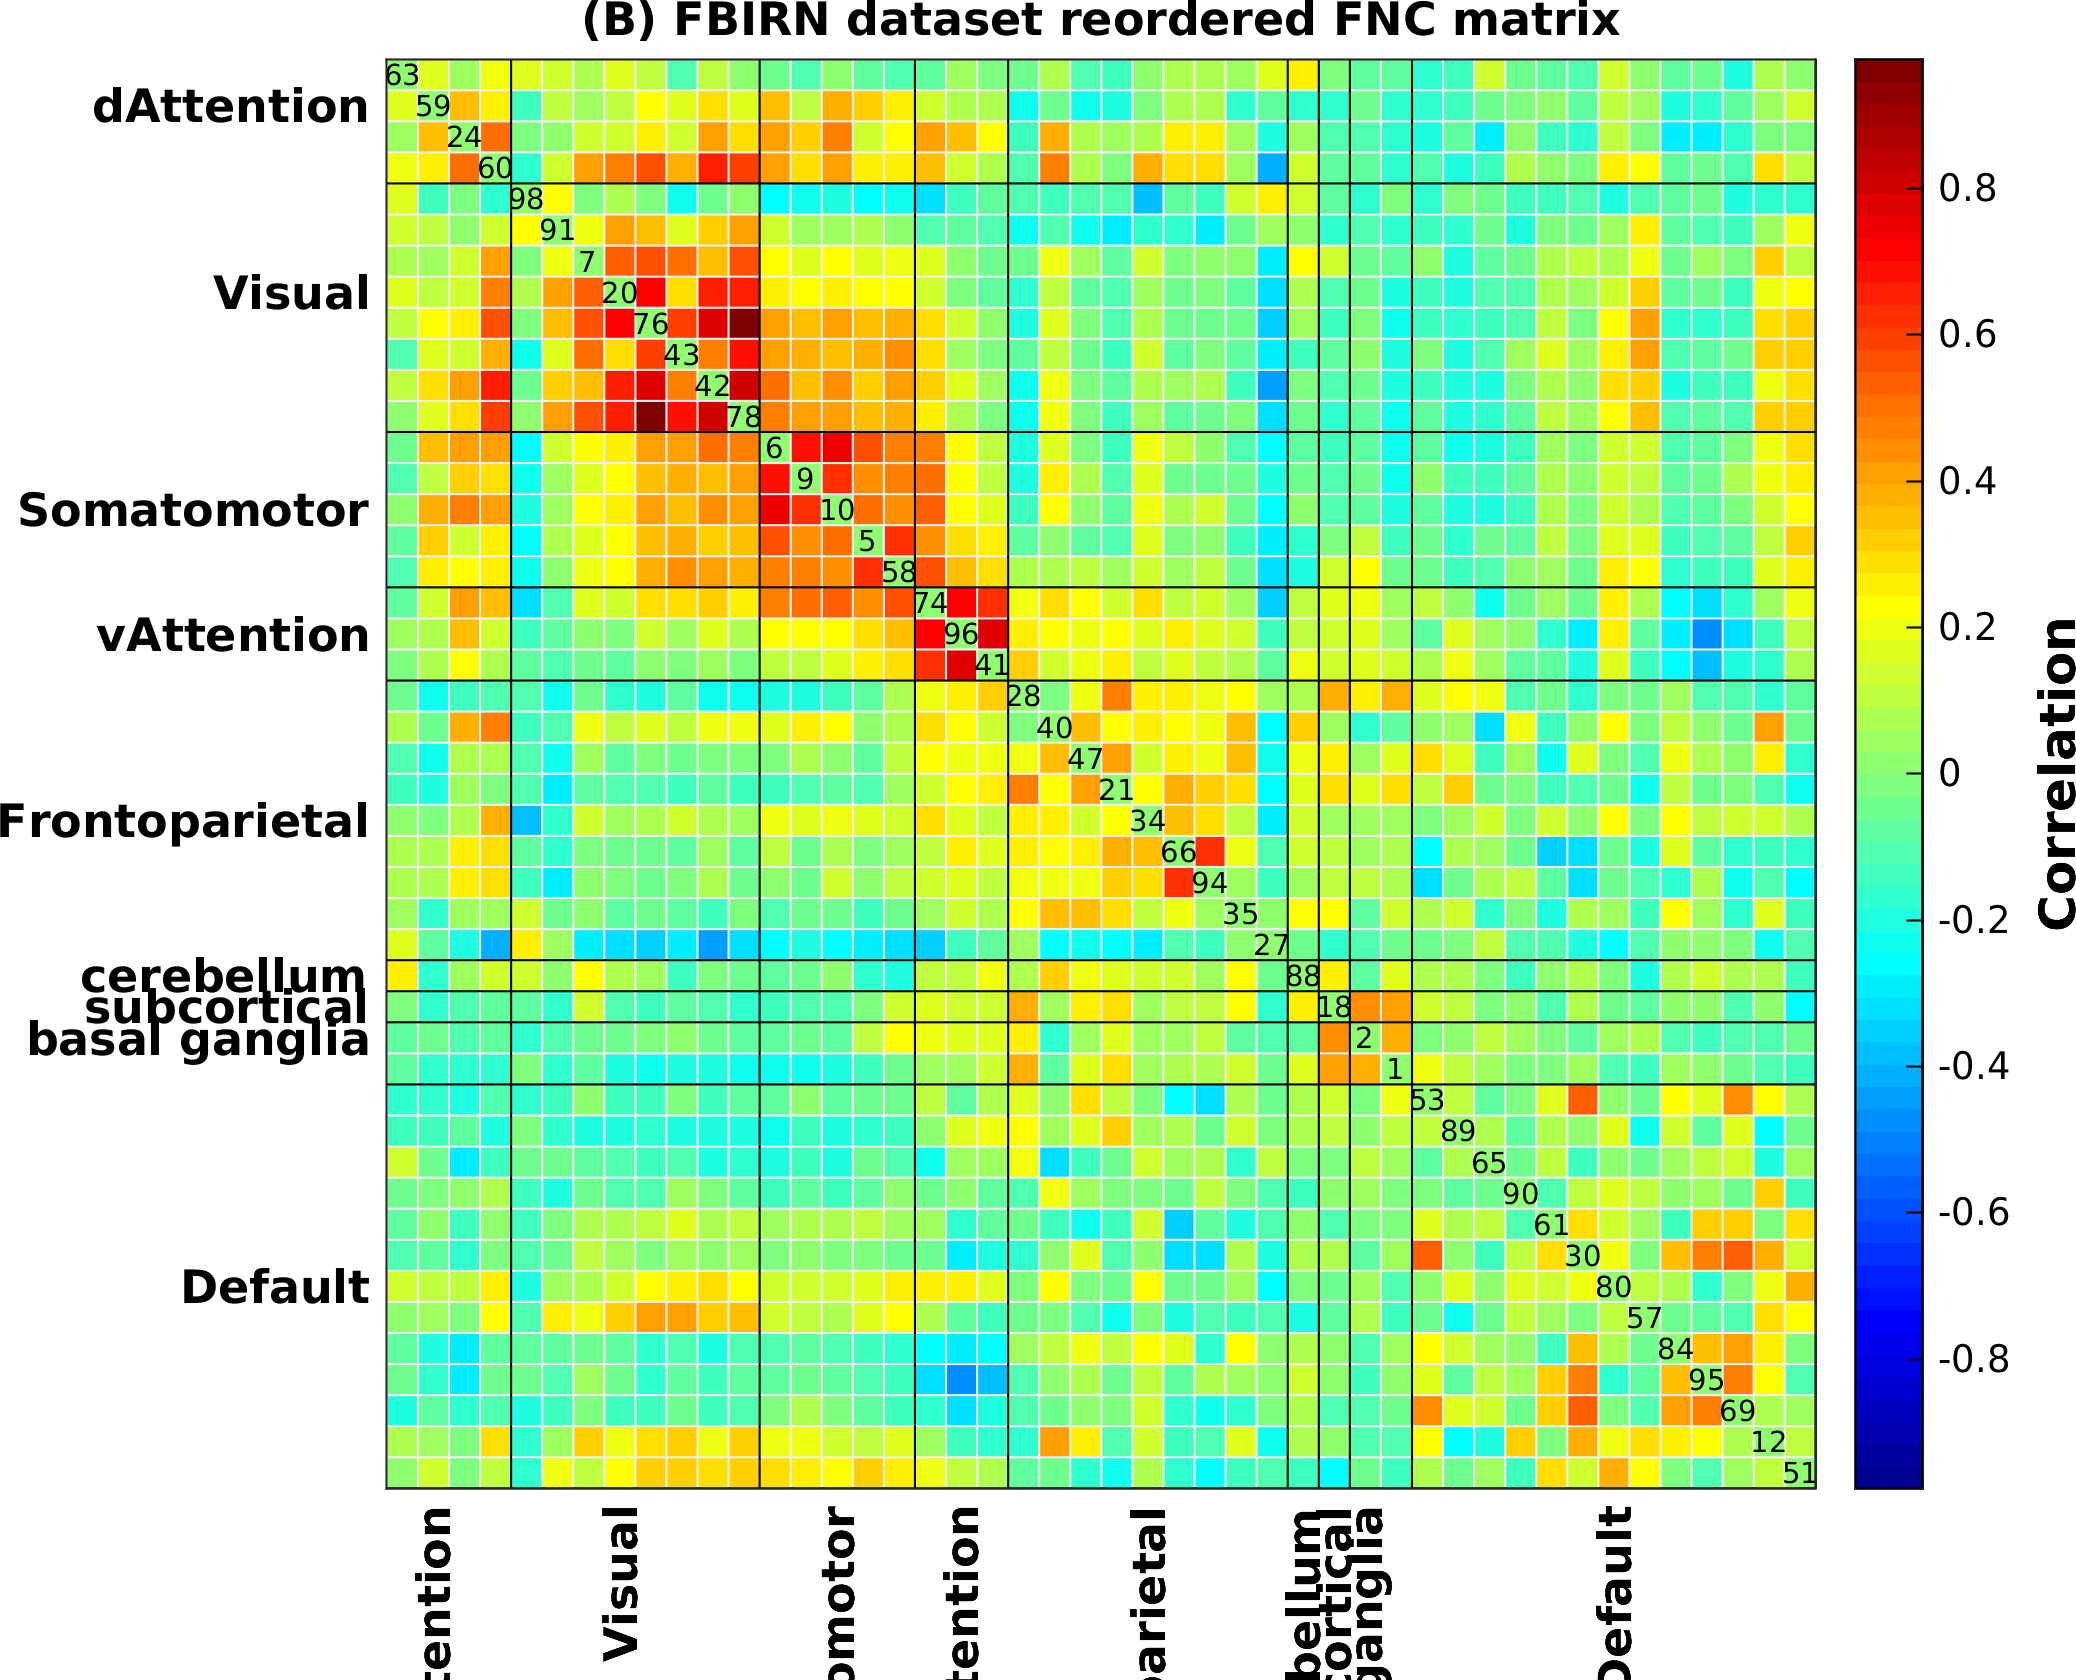
\includegraphics[width=\linewidth]{../../results/fbirn/fnc_reordered.pdf}
    \end{subfigure}
    \medskip
    \begin{subfigure}[t]{0.49\textwidth}
        \centering
        \includegraphics[width=\linewidth]{../../results/cobre/fnc_unsorted.pdf}
    \end{subfigure}
    \hfill
    \begin{subfigure}[t]{0.49\textwidth}
        \centering
        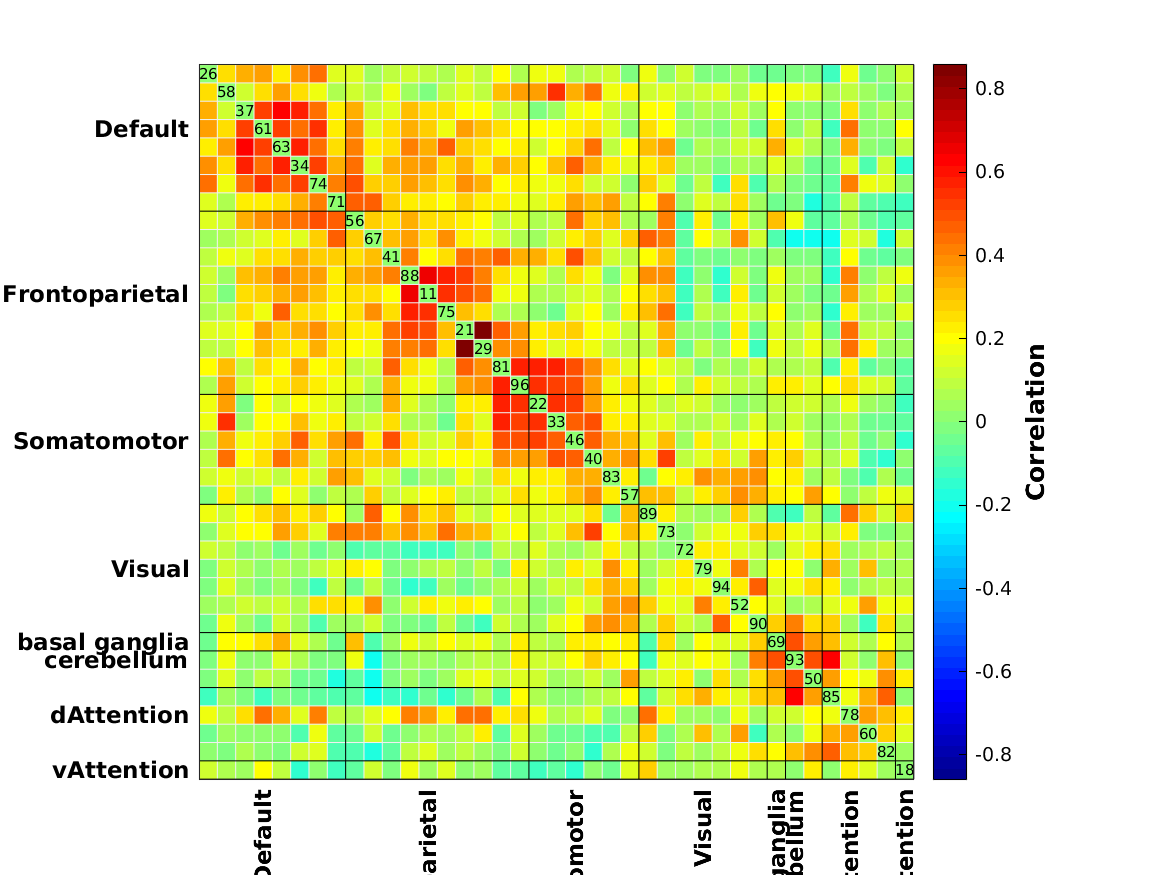
\includegraphics[width=\linewidth]{../../results/cobre/fnc_reordered.pdf}
    \end{subfigure}
    \caption{\label{fig:frog}Unsorted vs. automatically reordered \ac{FNC} matrices}
\end{figure}

\subsubsection{Parcellation \#2}

[figure]

[table of regions]

\subsubsection{Parcellation \#3}

[figure]

[table of regions]

\subsection{Reordering of FNC Matrix}

\section{Results}


\section{Discussion}

[motion estimate considerations]

[why some IC are mislabelled, eg. fbirn IC 12 is classified as default mode by Bucknerlab even though correlated with calcerine]

[why different atlas/parcellations chosen, pros/cons]

\begin{acronym}
    \acro{AAL}{Automated Anatomical Labeling}
    \acro{BSNIP}{Bipolar-Schizophrenia Network on Intermediate Phenotypes}
    \acro{COBRE}{Centers of Biomedical Research Excellence}
    \acro{CSF}{cerebrospinal fluid}
    \acro{fALFF}{fractional amplitude of low frequency fluctuation}
    \acro{FBIRN}{Function Biomedical Informatics Research Network}
    \acro{fMRI}{functional magnetic resonance imaging}
    \acro{FNC}{functional network connectivity}
    \acro{GIFT}{group ICA for fMRI toolbox}
    \acro{GSP}{Genomic Superstruct Project}
    \acro{HCP}{Human Connectome Project}
    \acro{IC}{independent component}
    \acro{ICA}{independent component analysis}
    \acro{RSN}{resting-state network}
    \acro{TC}{time course}
\end{acronym}

\bibliographystyle{apalike-refs}
\bibliography{sample}

\end{document}